\documentclass{article}

\usepackage{graphicx}
\usepackage{tikz}
\usepackage{tikzsymbols}
\usetikzlibrary{calc,patterns,shapes.geometric}
\pagestyle{empty}
\usepackage[margin=0pt]{geometry}
\geometry{papersize={14in,12in}}

\def\centerarc[#1](#2)(#3:#4:#5){\draw[#1] ($(#2)+({#5*cos(#3)},{#5*sin(#3)})$) arc (#3:#4:#5);}

\begin{document}
	\begin{figure}
		\centering
		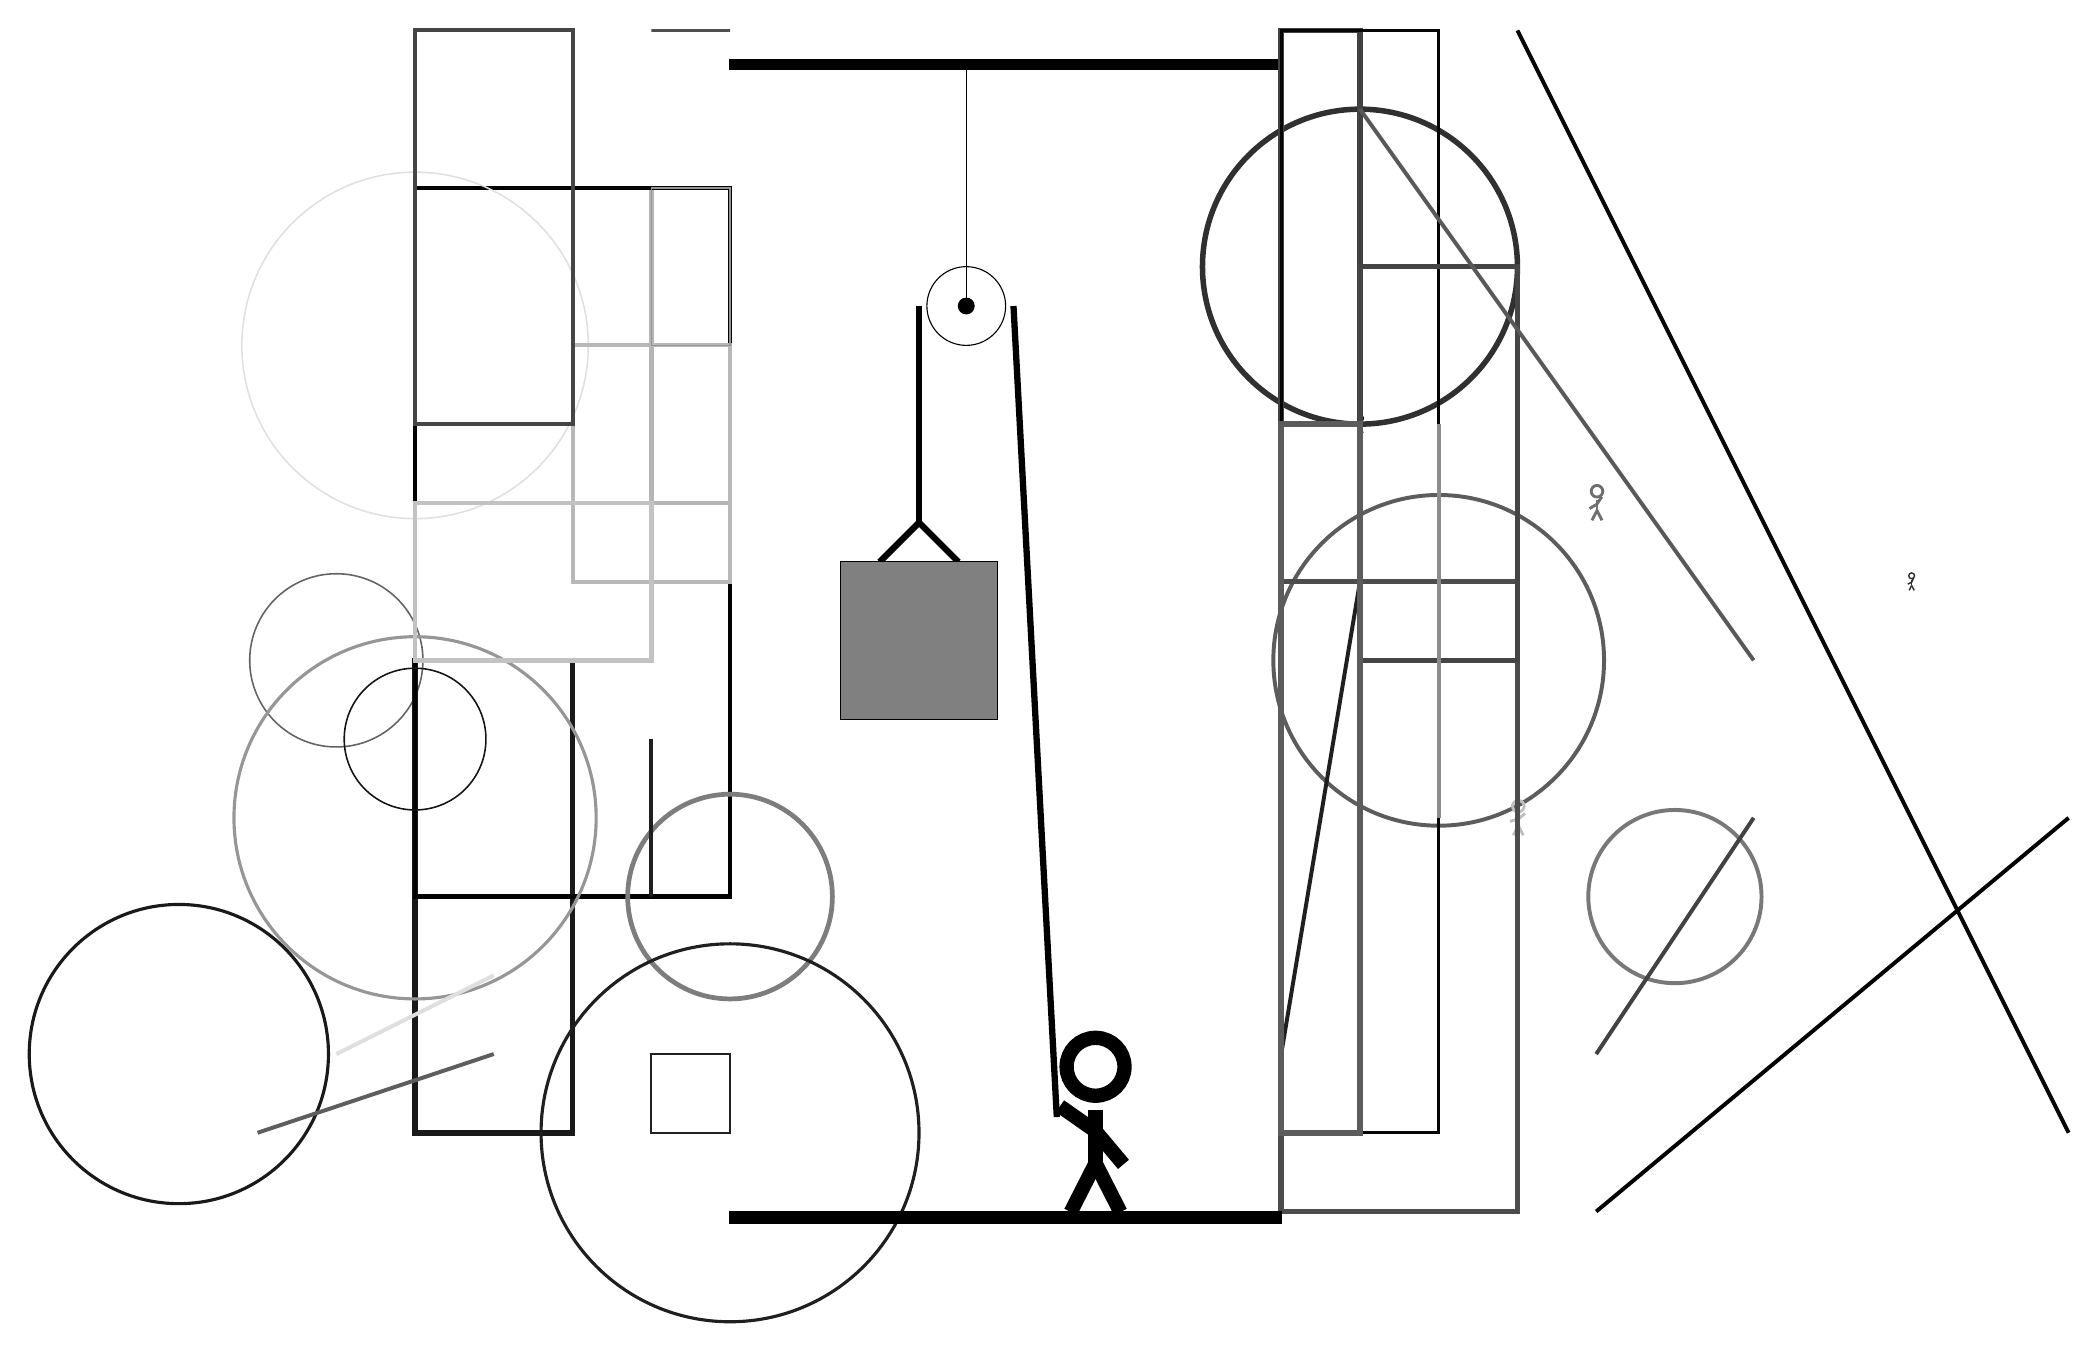
\begin{tikzpicture}
			%%%%% START %%%%%
			
			\draw[fill=black] (-2, 11.5) rectangle (5, 11.625);
			
			\draw (1, 8.5) circle (0.5);
			\draw[fill=black] (1, 8.5) circle (0.1);
			\draw (1, 11.5) -- (1, 8.5);
			
			\draw[line width=0.8mm] (-0.1, 5.25) -- (0.4, 5.75) -- (0.9, 5.25);
			\draw[fill=black!50] (-0.6, 5.25) rectangle (1.4, 3.25);
			
			\draw[line width=0.8mm] (0.4, 8.5) -- (0.4, 5.75);
			\centerarc[line width=0.8mm](1, 8.5)(0:180:0.6);
			\draw[line width=0.8mm](1.6, 8.5) -- (2.15, -1.8);
			
			\node[line width=0.3mm, color=black!92] at (6, 7) {\Strichmaxerl[1][18][82]};
			
			\draw[line width=0.6mm, color=black!29] (-2, 6) rectangle (-3, 10);
			\draw [line width=0.5mm, color=black!64](7, 4) circle (2.1);
			\draw [line width=0.7mm, color=black!81](6, 9) circle (2.0);
			\draw [line width=0.2mm, color=black!61](-7, 4) circle (1.1);
			\draw [line width=0.5mm, color=black!53](10, 1) circle (1.1);
			
			\node[line width=0.4mm, color=black!25] at (8, 2) {\Strichmaxerl[2][15][40]};
			
			\draw [line width=0.4mm, color=black!90](-9, -1) circle (1.9);
			\draw[line width=0.7mm, color=black!90] (-4, -2) rectangle (-6, 4);
			\draw[line width=0.7mm, color=black!74] (5, 12) rectangle (6, 7);
			\draw[line width=0.3mm, color=black!69] (-3, 12) rectangle (-2, 12);
			\draw[line width=0.6mm, color=black!99] (-2, 10) rectangle (-6, 1);
			\draw [line width=0.2mm, color=black!92](-6, 3) circle (0.9);
			
			\draw[line width=0.4mm, color=black!98] (5, 12) rectangle (7, -2);
			\draw[line width=0.3mm, color=black!87] (-3, -2) rectangle (-2, -1);
			\draw [line width=0.4mm, color=black!41](-6, 2) circle (2.3);
			
			\draw[line width=0.7mm, color=black!70] (5, 5) rectangle (8, -3);
			\draw[line width=0.6mm, color=black!73] (6, 9) rectangle (8, 4);
			\draw [line width=0.2mm, color=black!12](-6, 8) circle (2.2);
			\draw[line width=0.5mm, color=black!45](7, 7) -- (7, 2);
			\draw[line width=0.5mm, color=black!98](8, 12) -- (15, -2);
			
			\draw [line width=0.6mm, color=black!51](-2, 1) circle (1.3);
			\node[line width=0.2mm, color=black!57] at (9, 6) {\Strichmaxerl[2][31][57]};
			\draw[line width=0.5mm, color=black!74](9, -1) -- (11, 2);
			\draw[line width=0.5mm, color=black!28] (-2, 5) rectangle (-4, 8);
			
			\draw[line width=0.5mm, color=black!73] (-4, 7) rectangle (-6, 12);
			
			\draw[line width=0.5mm, color=black!88] (-3, 1) rectangle (-3, 3);
			\draw[line width=0.2mm, color=black!42] (-2, 8) rectangle (-3, 10);
			\draw[line width=0.5mm, color=black!13](-5, 0) -- (-7, -1);
			\draw [line width=0.4mm, color=black!88](-2, -2) circle (2.4);
			\draw[line width=0.5mm, color=black!65](6, 11) -- (11, 4);
			\node[line width=0.6mm, color=black!82] at (13, 5) {\Strichmaxerl[1][26][65]};
			\draw[line width=0.6mm, color=black!24] (-3, 4) rectangle (-6, 6);
			\draw[line width=0.5mm, color=black!88](5, -1) -- (6, 5);
			
			\draw[line width=0.7mm, color=black!64] (5, 7) rectangle (6, -2);
			\draw[line width=0.5mm, color=black!63](-5, -1) -- (-8, -2);
			\draw[line width=0.5mm, color=black!100](9, -3) -- (15, 2);
			
			\node at (2.6, -1.9) {\Strichmaxerl[10][-35][-50]};
			
			\draw[fill=black] (-2, -3) rectangle (5, -3.15);
			
			%%%%% END %%%%%
		\end{tikzpicture}
	\end{figure}	
\end{document}